\documentclass[../zavrsni.tex]{subfiles}

\begin{document}

\sloppy

\justifying

Postupkom opisanim u prošlom poglavlju generirani su izvještaji za ranije opisane algoritme koji su implementirani unutar FreeRTOS-a.
Iz izvještaja je potrebno dobiti grafove kako bi se vizualizirali i lakše interpretirali dobiveni rezultati. 
Za to je korišten programski jezik Python i u njemu uključen paket za crtanje grafičkih prikaza \texttt{matplotlib}. 
Sve simulacije su za određene uvjete pokrenute 20 puta, pa je zbog toga na grafovima prikazan prosjek dobivenih rezultata. 
Korišteni su skupovi s 5 zadataka. 

Na slici 5.1 prikazana je ovisnost kvavlitete usluge o faktoru opterećenja za sva tri opisana algoritma.

\begin{figure}[!htb]
    \center{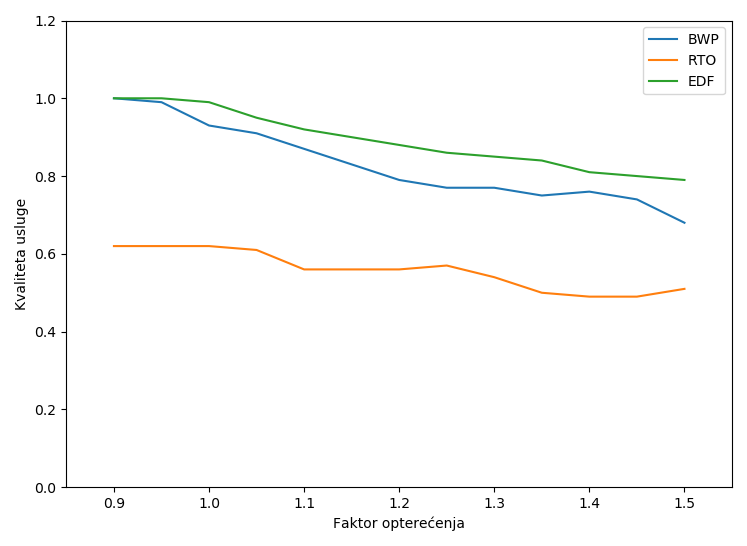
\includegraphics[width=\textwidth]
    {images/kvaliteta.png}}
    \caption{\label{fig:my-label} Usporedba algoritama EDF, RTO i BWP}
\end{figure}

U kontekstu \textit{skip-over} modela ublaženo-strogih uvjeta potrebno je usporediti algoritme RTO i BWP. 
%Graf dobiven iz podataka skupljenih simulacijama
%prikazan je na slici 5.3. Na grafu je prikazana ostvarena kvaliteta usluge u ovisnosti o faktoru opeterećenja.  
Vidljivo je da BWP algoritam za mala 
opterećenja ima puno veću kvalitetu usluge, koja opada kako opterećenje sustava raste. Kod algoritma RTO kvaliteta usluge je gotovo nepromjenjiva
u odnosu na faktor opterećenja i znatno niža od one kod algoritma BWP. 

Algoritam EDF ima najveću kvalitetu usluge, no izdvojen je od ostala dva jer nije primjenjiv za ublaženo-stroge
uvjete u sustavima za rad u stvarnom vremenu. Stoga je uz kvalitetu usluge, na posebnom grafu na slici 5.2 prikazan odnos broja kršenja 
postavljenih uvjeta u skip over modelu i ukupnog broja zadataka. Kršenje ublaženo-strogih uvjeta prikazuje se relativno u odnosu na broj 
poslova jer svaka simulacija ima različite vrijednosti perioda, a time i različit broj poslova.
Može se uočiti da porastom opetrećenja sustava, raste broj prekršenih uvjeta postavljenih nad skupom zadataka raspoređenih algoritmom EDF.
Za algoritme RTO i BWP svi postavljeni uvjeti su zadovoljeni, što je također prikazano na grafu.

\begin{figure}[!htb]
    \center{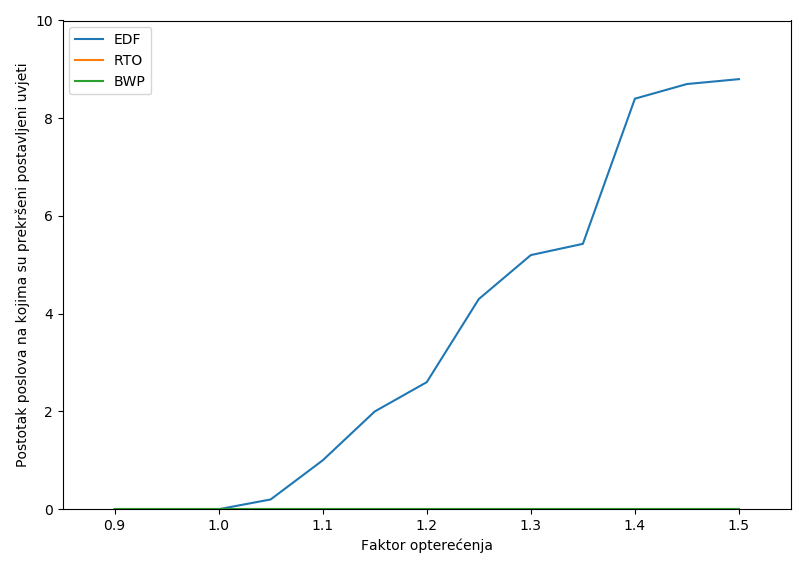
\includegraphics[width=\textwidth]
    {images/propusteno.png}}
    \caption{\label{fig:my-label} Postotak poslova na kojima je prekršen postavljen ublaženo strogi uvjet}
\end{figure}

\end{document}